\documentclass[../main.tex]{subfiles}

\begin{document}

\chapter{РОЗРОБКА І ТЕСТУВАННЯ БАГТРЕКЕРУ}

\section{Розробка багтрекінгової системи}

	На сьогоднішній день об'єктно-\linebreak[0]орієнтований підхід є одним із напрямків в проектуванні систем, що швидко розвивається. Прикладом можуть бути об'єктно-\linebreak[0]орієнтований аналіз — методологія розробки систем, запропонована Йорденом, об'єктно-орієнтоване проектування, об'єктно-\linebreak[0]орієнтоване програмування, реалізоване в численних компіляторах C++, Object Pascal, Borland Pascal, Smalltalk.
	
	Основу ООП складають три основні концепції: інкапсуляція, успадкування та поліморфізм. Одною з переваг ООП є краща модульність програмного забезпечення (тисячу функцій процедурної мови, в ООП можна замінити кількома десятками класів із своїми методами). Сьогодні багато мов програмування або підтримують ООП (PHP, Lua) або ж є цілком об'єктно-орієнтованими (зокрема, Java, C\#, C++, Python, Ruby та Objective-C, ActionScript 3, Swift, Vala).~\cite{oo_thought_process}
	
	На відміну від традиційних поглядів, коли програму розглядали як набір підпрограм, або як перелік інструкцій комп'ютеру, ООП програми можна вважати сукупністю об'єктів. Відповідно до парадигми об'єктно-\linebreak[0]орієнтованого програмування, кожний об'єкт здатний отримувати повідомлення, обробляти дані, та надсилати повідомлення іншим об'єктам. Кожен об'єкт — своєрідний незалежний автомат з окремим призначенням та відповідальністю.~\cite{object_oriented_analysis}
	
	ООП виникло в результаті розвитку ідеології процедурного програмування, де дані і підпрограми (процедури, функції) їх обробки формально не пов'язані. Для подальшого розвитку об'єктно-орієнтованого програмування велике значення мають поняття події (так зване подієво-орієнтоване програмування) і компоненти (компонентне програмування,~КОП).~\cite{oo_methods}
	
	Формування КОП від ООП відбулося, так само як формування модульного від процедурного програмування: процедури сформувалися в модулі — незалежні частини коду до рівня збірки програми, так об'єкти сформувалися в компоненти — незалежні частини коду до рівня виконання програми. Взаємодія об'єктів відбувається за допомогою повідомлень. Результатом подальшого розвитку ООП, мабуть, буде агентно-орієнтоване програмування, де агенти — незалежні частини коду на рівні виконання. Взаємодія агентів відбувається за допомогою зміни середовища, в якій вони знаходяться.
	
	Мовні конструкції, конструктивно не пов'язані безпосередньо з об'єктами, але необхідні їм для їх безпечної (виняткові ситуації, перевірки) та ефективної роботи, інкапсулюються від них в аспекти (в~аспектно-\linebreak[0]орієнтованому програмуванні). Суб'єктно-орієнтоване програмування розширює поняття об'єктів шляхом забезпечення більш уніфікованого і незалежної взаємодії об'єктів. Може бути перехідною стадією між ООП та агентним програмуванням в частині самостійної їх взаємодії.
	
	\subsection{Обґрунтування вибору засобів реалізації багтрекеру}
		Для реалізації серверної частини програмного комплексу багтрекінгової системи було використано:
		\begin{enumerate}
			\item Swagger -- формалізована специфікація і екосистема безлічі інструментів, що надає інтерфейс між front-end системами, кодом бібліотек низького рівня і комерційними рішеннями у вигляді API. Разом з тим, специфікація побудована таким чином, що не залежить від мов програмування, і зручна у використанні як людиною, так і машиною \cite{swagger}.
			\item REST -- підхід до архітектури мережевих протоколів, які забезпечують доступ до інформаційних ресурсів.
			\item JSON -- текстовий формат обміну даними між комп'ютерами. Базується на тексті, може бути прочитаним людиною. Формат дозволяє описувати об'єкти та інші структури даних.
			\item Node.js -- платформа з відкритим кодом для виконання високопродуктивних мережевих застосунків, написаних мовою JavaScript.
			\item JavaScript -- динамічна, об'єктно-орієнтована мова програмування. Реалізація стандарту ECMAScript.
			\item MariaDB -- реляційна система керування базами даних, створена на початку 2009 як відгалуження (форк) MySQL.
		\end{enumerate}
		
		Вибір Swagger'у в ролі фреймворку специфікації обумовлений тим, що на даний момент це єдиний абсолютно безкоштовний та підтримуваний фреймворк даного типу. Його використання дозволило значно пошвидшити розробку системи, надаючи методи з генерації робочих моделей даних та каркасів роботи з ними для конкретних платформ розробки. Щодо призначення, OpenAPI розглядається як універсальний інтерфейс для користувачів (клієнтів) по взаємодії з сервісами (серверами). Якщо спроектована специфікація для деякого сервісу, то на її підставі можна генерувати вихідний код для бібліотек клієнтських додатків, текстову документацію для користувачів, варіанти тестування та ін. Для цих дій є великий набір інструментів для різних мов програмування і платформ.
		
		Swagger специфікація не залежить від мови програмування, і може бути використана поза протоколом HTTP. OpenAPI одночасно застосовується для клієнта, сервера і відповідної документації інтерфейсу, створеного відповідно до REST. Специфікація декларативна, і тому може бути використана клієнтами без знань особливостей серверної реалізації. При цьому працювати з OpenAPI можуть як розробники, так і рядові користувачі через готові інструменти та інтерфейси, що надаються. В ролі формату обміну даними використовується XML або JSON, але за потреби може бути обраний й інший механізм серіалізації.
		
		В якості стилю обміну даними між клієнотом та сервером було вибрано REST з таких причин:
		\begin{enumerate}
			\item Легкість.
			\item Простота в обслуговуванні.
			\item Масштабованість і гнучкість.
			\item Ефективність і швидкість.
			\item Висока продуктивність.
			\item Споживання низької кількості трафіку.
			\item Можливість використання без дорогих сторонніх інструментів.
		\end{enumerate}
		Окрім цього, в основі REST закладено принципи функціонування Всесвітньої павутини і, зокрема, можливості HTTP. Філдінг розробив REST паралельно з HTTP 1.1 базуючись на попередньому протоколі HTTP 1.0.
		
		REST, як і кожен архітектурний стиль відповідає ряду архітектурних обмежень. Це гібридний стиль який успадковує обмеження з інших архітектурних стилів.
		
		Перша архітектура від якої він успадковує обмеження — це клієнт-серверна архітектура. Її обмеження вимагає розділення відповідальності між компонентами які займаються зберіганням та оновленням даних (сервером) і тими компонентами які займаються відображенням даних на інтерфейсі користувача та реагування на дії з цим інтерфейсом (клієнтом). Таке розділення дозволяє компонентам еволюціонувати незалежно.
		
		Наступним обмеженням є те, що взаємодії між сервером та клієнтом не~мають стану, тобто кожен запит містить всю необхідну інформацію для його обробки, і не~покладається на те, що сервер знає щось з попереднього запиту. Таким чином, наприклад дані про стан сесії (користувача який аутентифікувався) зберігаються на клієнті, і передаються з кожним запитом. Це покращує масштабовність, бо сервер після закінчення обробки запиту може звільнити всі ресурси задіяні для цієї операції, без жодного ризику втратити цінну інформацію. Також спрощується моніторинг і зневадження, бо для того, аби розібратись, що відбувається в певному запиті, досить подивитись лише на той один запит. Збільшується надійність, бо помилка в одному запиті не~зачіпає інші.
		
		Мінусом цього обмеження є те, що знижується продуктивність, через те що в кожен запит тепер доводиться додавати дані сесії з клієнта. Також збереження стану на різних клієнтах важче підтримувати, бо реалізації клієнтів можуть відрізнятись, в той час як середовище сервера повністю під контролем розробника.
		
		Додатковим обмеженням стилю REST є те, що системи написані в цьому стилі повинні підтримувати кешування, тобто дані які передаються між сервером та клієнтом повинні містити інформацію про те, чи можна їх кешувати, і якщо можна, то як довго. Це дозволяє збільшувати продуктивність, уникаючи зайвих запитів, але також зменшує надійність системи, через те, що дані в кеші можуть бути застарілі.
		
		Рання архітектура веб, створена Тімом Бернерсом-Лі, відповідала цим трьом обмеженням — клієнт-сервер без стану з підтримкою кешування. Проте стиль REST додає ще додаткові обмеження.
		
		Всі компоненти в архітектурі REST підтримують однорідний інтерфейс. Це зменшує зв'язність між компонентами і сервісами які вони надають і дозволяє нескладно змінювати компоненти при потребі. Це досягається кількома точнішими обмеженнями:
		
		\begin{itemize}
			\item ідентифікація ресурсів;
			\item маніпуляція ресурсами через представлення;
			\item самоописові повідомлення;
			\item гіпермедіа як рушій стану застосунку.
		\end{itemize}
		
		Наступним обмеженням для REST є поділ на шари абстракції. Кожен компонент потрапляє в якийсь шар, і спілкується лише з компонентами в шарі під ним або в шарі над ним. Обмежнення знання системи одним шаром зменшує складність компонентів.
		
		Останнім архітектурним обмеженням в REST є те, що клієнти повинні дозволяти розширювати свою функціональність, дозволяючи завантаження додаткового коду (code on demand[en]) у~формі аплетів чи скриптів. Це~спрощує клієнти, дозволяючи не~реалізовувати всі необхідні функції попередньо. Щоправда це необов'язкове обмеження, і якщо воно не дає переваг для конкретного застосування, то його не обов'язково реалізовувати. Наприклад, дозвіл завантаження стороннього коду може бути не бажаним з точки зору безпеки.
		
		Компоненти REST системи спілкуються, передаючи один одному представлення ресурсу в форматі, що обирається з оновлюваного набору стандартних форматів даних. Формат обирається динамічно відповідно до бажань компонента-клієнта і можливостей сервера. Чи представлення має той самий формат, що й сам ресурс, чи є результатом якогось перетворення\nolinebreak[2] — це деталь реалізації, яка ховається за інтерфейсом.
		
		Ресурс — це ключовий елемент даних в REST. Ресурсом може бути що завгодно, що можна назвати: якийсь документ (наприклад додаток до звіту), динамічне значення (наприклад інформація щодо проекту), щось з реального світу (наприклад інформація щодо учасника проекту).
		
		Для того, щоб посилатись на ресурси, використовуються ідентифікатори ресурсів. Компонент, який надав ресурсу ідентифікатор і дозволяє звертатись до нього за цим ідентифікатором, відповідає за збереження функції приналежності незмінною. Якість ідентифікатора залежить від якості компонента, який цей ідентифікатор надає, тому деякі ідентифікатори стають «мертвими посиланнями», коли інформацію переміщують або знищують.
		
		В якості формату обміну даними між клієнтом та сервером було вибрано JSON з таких причин:
		\begin{enumerate}
			\item Малий розмір повідомлення.
			\item Гарно структурована інформація в документі.
			\item Легко розрізняти типи даних.
			\item Можна легко розрізняти окремі предмети і колекції розміром в один елемент.
			\item Легко передати null-значення.
			\item Легко обробляти за допомогою JavaScript.
		\end{enumerate}
		
		За рахунок своєї лаконічності в порівнянні з XML, формат JSON може бути більш придатним для серіалізації складних структур.
		
		JSON будується на двох структурах:
		\begin{enumerate}
			\item Набір пар ім'я/значення. У різних мовах це реалізовано як об'єкт, запис, структура, словник, хеш-таблиця, список з ключем або асоціативний масив.
			\item Впорядкований список значень. У багатьох мовах це реалізовано як масив, вектор, список, або послідовність.
		\end{enumerate}
		
		Це універсальні структури даних. Теоретично всі сучасні мови програмування підтримують їх у тій чи іншій формі. Оскільки JSON використовується для обміну даними між різними мовами програмування, то є сенс будувати його на цих структурах.
		
		У JSON використовуються такі їхні форми:
		\begin{enumerate}
			\item Об'єкт — це послідовність пар ім'я/значення. Об'єкт починається з символу \{ і закінчується символом \}. Кожне значення слідує за : і пари ім'я/значення відділяються комами.
			\item Масив — це послідовність значень. Масив починається символом [ і закінчується символом ]. Значення відділяються комами.
			\item Значення може бути рядком в подвійних лапках, або числом, або логічними true чи false, або null, або об'єктом, або масивом. Ці\nolinebreak[3] структури можуть бути вкладені одна в одну.
			\item Рядок — це послідовність з нуля або більше символів юнікода, обмежена подвійними лапками, з використанням escape-\linebreak[0]послідовностей, що починаються із зворотної косої риски (backslash). Символи представляються простим рядком.
		\end{enumerate}
		
		Тип Рядок (String) дуже схожий на String в мовах C і Java. Число теж дуже схоже на C- або Java-число, за винятком того, що вісімкові та шістнадцяткові формати не використовуються. Пропуски можуть бути вставлені між будь-якими двома лексемами.
		
		Node.js було вибрано у ролі середовища виконання серверного додатку тому, що це найбільш популярна, стабільна та ефективна реалізація серверного середовища виконання JavaScript коду.\pagebreak[2] % фактически чтоб уменьшить риск отрыва следующего абзаца (являющегося по сути заголовком списка) от самогО списка. Увы, поставить там \nopagebreak не~работает
		
		Node.js характеризується такими властивостями:
		\begin{enumerate}
			\item Асинхронна однопотокова модель виконання запитів.
			\item Неблокуючий ввід/вивід.
			\item Система модулів CommonJS.
			\item Рушій JavaScript Google V8.
		\end{enumerate}
		
		Node.js призначений для відокремленого виконання високопродуктивних мережних застосунків на мові JavaScript. Функції платформи не обмежені створенням серверних скриптів для веб, платформа може використовуватися і для створення звичайних клієнтських і серверних мережевих програм. Для забезпечення виконання JavaScript-коду використовується розроблений компанією Google рушій V8.
		
		Для забезпечення обробки великої кількості паралельних запитів у Node.js використовується асинхронна модель запуску коду, заснована на обробці подій в неблокуючому режимі та визначенні обробників зворотніх викликів (callback). Як способи мультиплексування з'єднань підтримується epoll, kqueue, /dev/poll і select. Для мультиплексування з'єднань використовується бібліотека libuv, для створення пулу потоків (thread pool) задіяна бібліотека libeio, для виконання DNS-запитів у неблокуючому режимі інтегрований c-ares. Всі системні виклики, що спричиняють блокування, виконуються всередині пула потоків і потім, як і обробники сигналів, передають результат своєї роботи назад через неіменовані канали~(pipe). % to avoid too short last line
		
		Для розширення функціональності застосунків на базі Node.js підготовлена велика колекція модулів, в якій можна знайти реалізацію HTTP, SMTP, XMPP, DNS, FTP, IMAP, POP3 серверів і клієнтів, модулі для інтеграції з різними веб-фреймворками, обробники WebSocket і AJAX, конектори до СУБД (MySQL, PostgreSQL, SQLite, MongoDB), шаблонізатори, CSS-рушії, реалізації криптоалгоритмів і систем авторизації (наприклад, OAuth), XML-парсери.
		
		JavaScript було вибрано як мову реалізації серверної частини з таких причин:
		\begin{enumerate}
			\item Можливість використовувати одну й ту саму мову програмування як на сервері, так і на клієнті.
			\item Висока швидкість у зв'язці з Node.js.
			\item Підтримка JSON об'єктів без необхідності в створенні будь-яких моделей для опису повідомлень.
			\item Можливість прямого зв'язування зі Swagger специфікацією без потреби в написанні додаткового коду.
			\item Динамічна типізація, що дозволяє розроблювати систему швидше та додає їй гнучкості.
		\end{enumerate}
		
		JavaScript класифікують як прототипну (підмножина об'єктно-\linebreak[0]орієнтованої) скриптову мову програмування з динамічною типізацією. Окрім прототипної, JavaScript також частково підтримує інші парадигми програмування (імперативну та частково функціональну) і деякі відповідні архітектурні властивості, зокрема: динамічна та слабка типізація, автоматичне керування пам'яттю, прототипне наслідування, функції як об'єкти першого класу.
		
		Незважаючи на схожість назв, мови Java та JavaScript є двома різними мовами, що мають відмінну семантику, хоча й мають схожі риси в стандартних бібліотеках та правилах іменування. Синтаксис обох мов отриманний «у спадок» від мови С, але семантика та дизайн JavaScript є результатом впливу мов Self та Scheme.
		
		JavaScript має низку властивостей об'єктно-орієнтованої мови, але завдяки концепції прототипів підтримка об'єктів в ній відрізняється від традиційних мов ООП. Крім того, JavaScript має ряд властивостей, притаманних функціональним мовам — функції як об'єкти першого класу, об'єкти як списки, каррінг, анонімні функції, замикання (closures) — що додає мові додаткову гнучкість.
		
		JavaScript має C-подібний синтаксис, але в порівнянні з мовою С має такі корінні відмінності:
		\begin{enumerate}
			\item Об'єкти, з можливістю інтроспекції і динамічної зміни типу через механізм прототипів.
			\item Функції як об'єкти першого класу.
			\item Обробка винятків.
			\item Автоматичне приведення типів.
			\item Автоматичне прибирання сміття.
			\item Анонімні функції.
		\end{enumerate}
		
		JavaScript містить декілька вбудованих об'єктів: Global, Object, Error, Function, Array, String, Boolean, Number, Math, Date, RegExp. Крім того, JavaScript містить набір вбудованих операцій, які, строго кажучи, не~обов'язково є функціями або методами, а також набір вбудованих операторів, що управляють логікою виконання програм. Синтаксис JavaScript в основному відповідає синтаксису мови Java (тобто, зрештою, успадкований від C), але спрощений порівняно з ним, щоб зробити мову сценаріїв легкою для вивчення.
	
	\subsection{Опис структурної схеми багтрекеру}
		\begin{figure}[H]
			\centering
			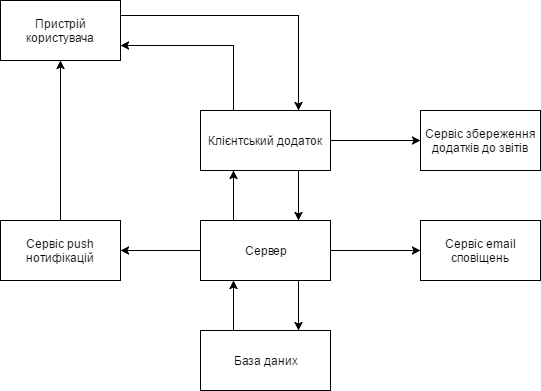
\includegraphics[width=0.75\textwidth]{4_structural_scheme}
			\caption{Структурна схема функціювання багтрекеру}
			\label{structural_scheme}
		\end{figure}
	
		Враховуючи клієнт-серверу природу багтрекінгових систем, розроблена вимагає для своєї роботи наявність декількох вузлів (зображених на схемі \ref{structural_scheme}):
		\begin{enumerate}
			\item Пристрій користувача -- пристрій, за допомогою якого користувач використовує клієнтський додаток.
			\item Клієнтський додаток -- програма, що дозволяє взаємодіяти з іншими складовими багтрекінгової системи.
			\item Сервер -- центральний вузол всієї системи, потрібен для обробки інформації від клієнтських додатків.
			\item База даних -- забезпечує збереження інформації в системі.
			\item Сервіс push нотифікацій -- забезпечує пряме сповіщення користувачів системи щодо змін даних в звітах.
			\item Сервіс email нотифікацій -- забезпечує сповіщення користувачів системи щодо змін даних в звітах за допомогою електронних листів.
			\item Сервіс збереження додатків до звітів -- забезпечує зберігання додаткової інформації звіту.
		\end{enumerate}
	
	\subsection{Опис логічної схеми багтрекінгової системи}
		Для роботи з багтрекінговою системою обов'язковою умовою є авторизація. Неавторизований користувач в системі має право лише на операції авторизації або реєстрації.
		
		\subparagraph{Авторизація.}
			Для авторизації користувач повинен здійснити наступні кроки:
			\begin{enumerate}
				\item Ввести логін.
				\item Ввести пароль.
			\end{enumerate}

			\begin{figure}[H]
				\centering
				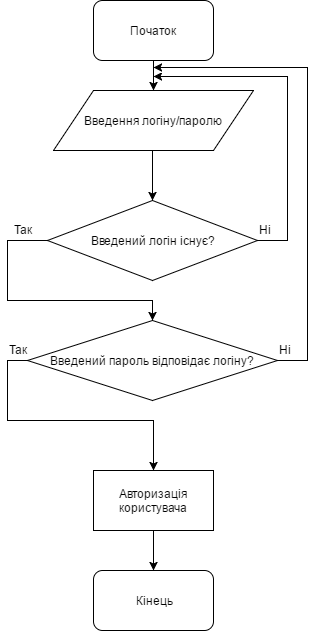
\includegraphics[width=0.4\textwidth]{4_login_flow}
				\caption{Блок-схема авторизації користувача багтрекеру}
				\label{flowchart_login}
			\end{figure}

			У випадку введення неіснуючого логіну або неправильного паролю користувач буде змушений ввести ці дані заново до тих пір, доки сервер не підтвердить правильніть введених даних. Блок-схему авторизації користувача багтрекеру зображено на рис.~\ref{flowchart_login}.
		
		\subparagraph{Реєстрація.}
			Для реєстрації користувач повинен здійснити наступні кроки:
			\begin{enumerate}
				\item Ввести бажаний логін.
				\item Ввести бажаний пароль.
			\end{enumerate}
			
			У випадку вибору зайнятого логіну або занадто слабкого паролю користувач буде змушений ввести ці дані заново до тих пір, доки сервер не підтвердить, що вибраний логін є вільним, а пароль є достатньо сильним. Блок-схему реєстрації користувача багтрекеру зображено на рис.~\ref{flowchart_signup}.
			
			\begin{figure}[H]
				\centering
				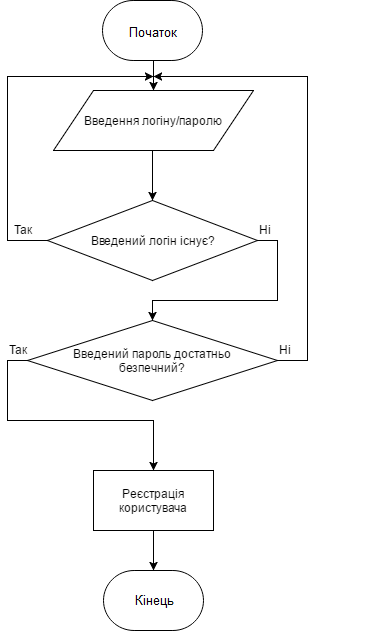
\includegraphics[width=0.4\textwidth]{4_signup_flow}
				\caption{Блок-схема реєстрації користувача багтрекеру}
				\label{flowchart_signup}
			\end{figure}
		
		\subparagraph{Створення проекту.}
			Для створення нового проекту користувач повинен здійснити наступні кроки:
			\begin{enumerate}
				\item Ввести назву проекту.
				\item Ввести которкий опис проекту.
				\item (Опціонально) ввести повний опис проекту.
			\end{enumerate}
			
			У випадку вибору уже існуючої назви проекту або відсутності короткого опису проекту, користувач буде змушений ввести ці дані заново до тих пір, доки сервер не підтвердить, що проекту з такою назвою ще не існує та короткий опис присутній. Блок-схему створення проекту в багтрекері зображено на рис.~\ref{flowchart_project_creation}.
			
			\begin{figure}[H]
				\centering
				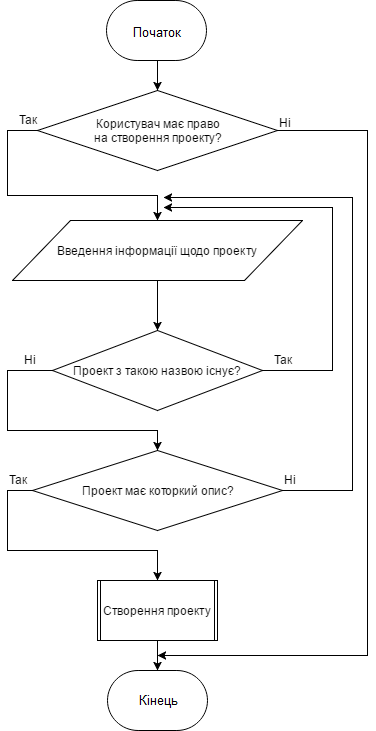
\includegraphics[width=0.5\textwidth]{4_project_creation_flow}
				\caption{Блок-схема створення проекту в багтрекері}
				\label{flowchart_project_creation}
			\end{figure}
		
		\subparagraph{Створення звіту.}
			Для створення нового звіту користувач повинен здійснити наступні кроки:
			\begin{enumerate}
				\item Ввести которткий опис проблеми.
				\item Обрати тип проблеми.
			\end{enumerate}
			
			У випадку відсутності короткого опису проблеми або не обраного типу, користувач буде змушений ввести ці дані заново до тих пір, доки сервер не підтвердить, що короткий опис проблеми присутній, а тип обрано.
			
			\begin{figure}[H]
				\centering
				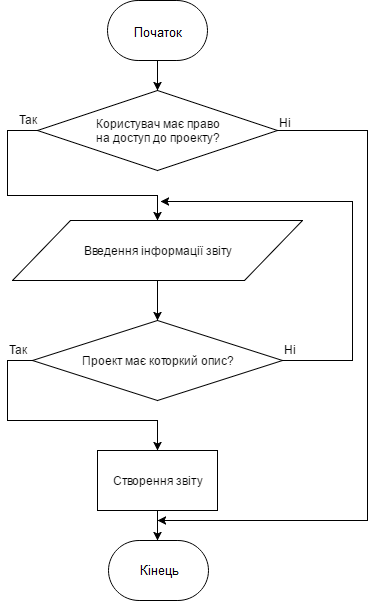
\includegraphics[width=0.5\textwidth]{4_issue_creation_flow}
				\caption{Блок-схема створення звіту в багтрекінговій системі}
				\label{flowchart_issue_creation}
			\end{figure}
			
			Також, за бажанням, користувач може виконати одну з таких дій:
			\begin{enumerate}
				\item Обрати відповідального за проблему (якщо володіє відповідним правом).
				\item Прикріпити додатки.
				\item Ввести повний опис проблеми.
				\item Прикріпити додаткову інформацію.
			\end{enumerate}
			
			Блок-схему створення звіту в багтрекінговій системі зображено на рис.~\ref{flowchart_issue_creation}.

	\subsection{Розробка бази даних багтрекеру}
		База даних системи, як зображено на схемах \ref{db_concept}, \ref{db_logical} та \ref{db_physical}, складається з таких основних сутностей:
		\begin{enumerate}
			\item User -- сутність, що уособлює користувача системи.
			\item Project -- сутність, що уособлює проект в системі.
			\item Issue -- сутність, що уособлює звіт в системі.
		\end{enumerate}
		
		Серед допоміжних сутностей, що забезпечують роботу системи, є такі:
		\begin{enumerate}
			\item Project Member -- сутність, що забезпечує можливість установлення факту участі користувача в проекті.
			\item Permission -- сутність, що забезпечує обмеження можливостей користувачів.
			\item Role -- сутність, що забезпечує можливість групування дозволів на певні дії для забезпечення підтримки рольової структури проектів.
			\item Project Issue -- сутність, що забезпечує можливість нумерації звітів як на рівні всієї системи, так і на рівні окремого проекту.
			\item Issue Type -- сутність, що забезпечує можливість вказування типу звіту.
			\item Issue Status -- сутність, що забезпечує можливість вказувати статус звіту.
			\item Issue Attachment -- сутність, що забезпечує можливість прикріплення додатку до звіту.
		\end{enumerate}
		
		\begin{figure}[H]
			\centering
			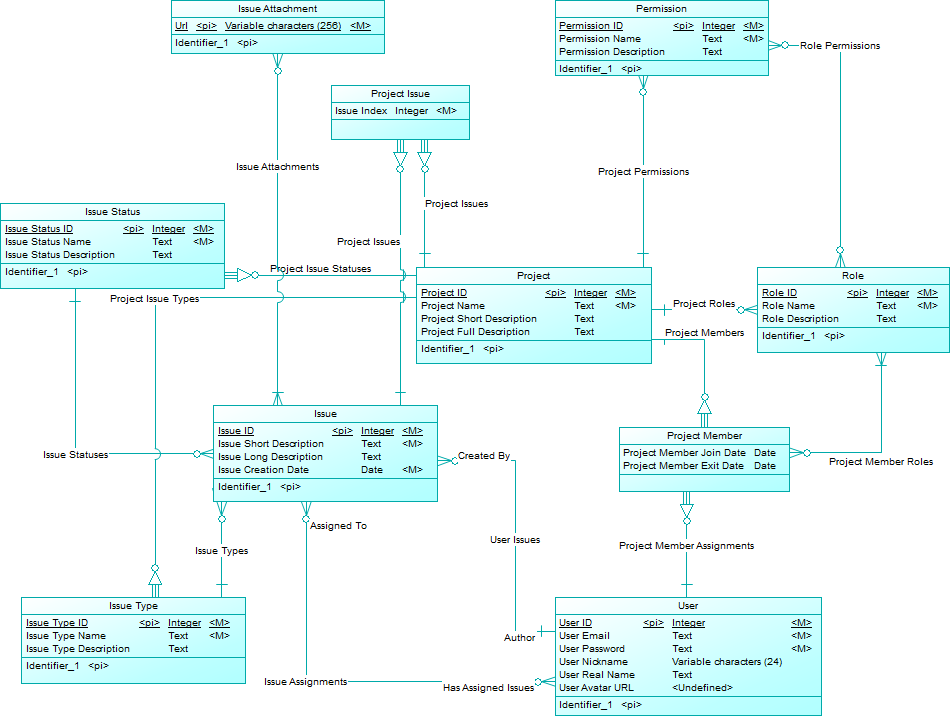
\includegraphics[width=1\textwidth]{4_db_concept}
			\caption{Концептуальна модель бази даних багтрекеру}
			\label{db_concept}
		\end{figure}
		
		Реалізація багтрекінгової системи потребує пред'являє високі вимоги до побудови бази даних. Для реалізації гнучкої системи, використання зв'язку ''багато до багатьох'' є необхідною умовою. Концептуальна модель не відображає реальної будови майбутньої бази даних. В реальній базі даних окрім таблиць для вже зазначених вище сутностей будуть ще й такі з'єднувальні таблиці (див. рис. \ref{db_logical}, \ref{db_physical}):
		
		\begin{enumerate}
			\item Issue Attachments -- таблиця, що з'єднує звіти з їх додатками.
			\item Role Permissions -- таблиця, що з'єднує ролі з дозволеними діями. Є необхідною складовою реалізації ролей учасників проектів.
			\item Project Member Roles -- таблиця, що з'єднує учасника проекту з присвоєними йому ролями. Є необхідною складовою реалізації ролей учасників проектів.
			\item Issue Assignments -- таблиця, що з'єднує звіт з відповідальним за нього членом команди. Є необхідною складовою реалізації можливості присвоєння декількох відповідальних за звіт осіб.
		\end{enumerate}
		
		\begin{figure}[H]
			\centering
			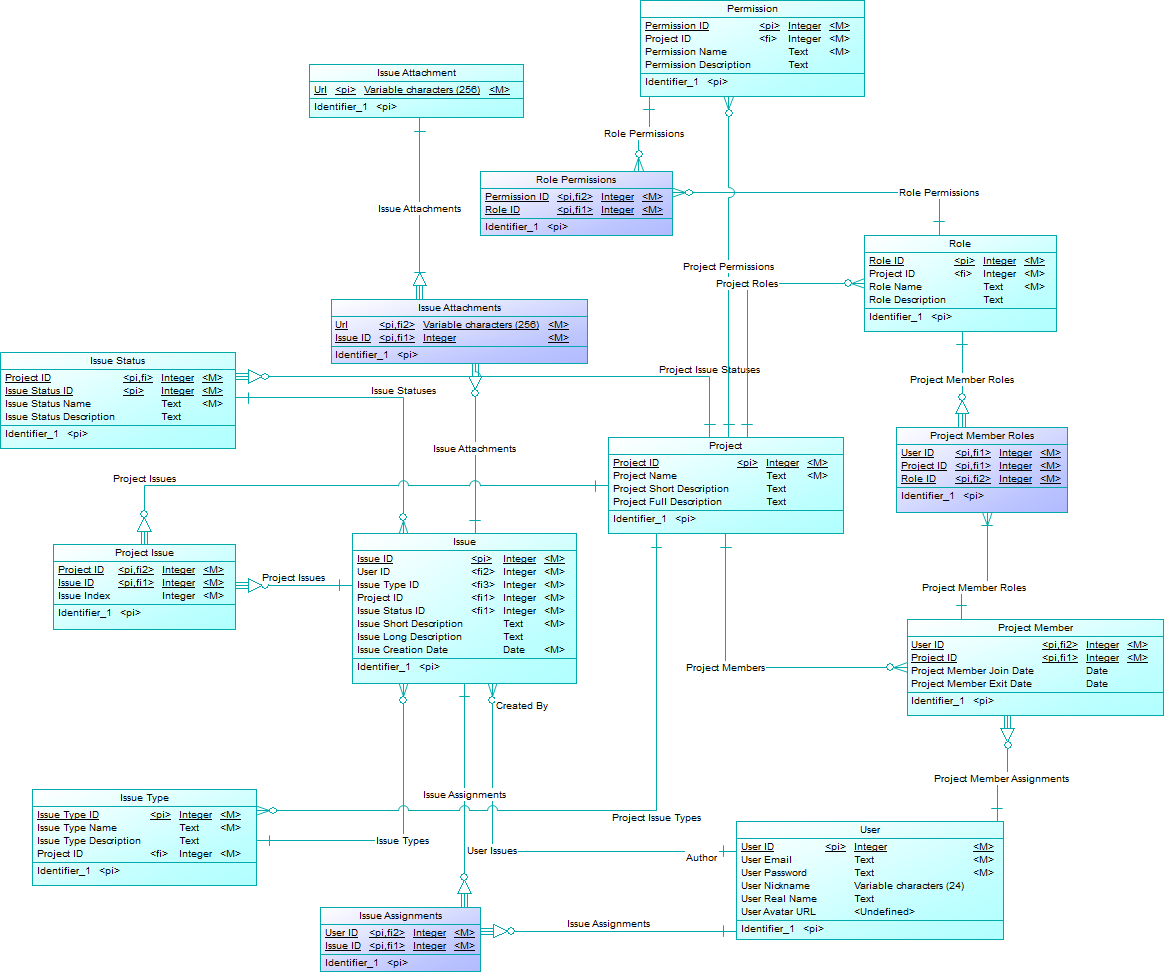
\includegraphics[width=1\textwidth]{4_db_logical}
			\caption{Логічна модель бази даних багтрекеру}
			\label{db_logical}
		\end{figure}
		
		Для представлення бази даних у найбільш прийнятному для імплеметації форматі було також створено фізичну схему бази даних. (див. рис. \ref{db_physical})
		
		\begin{figure}[H]
			\centering
			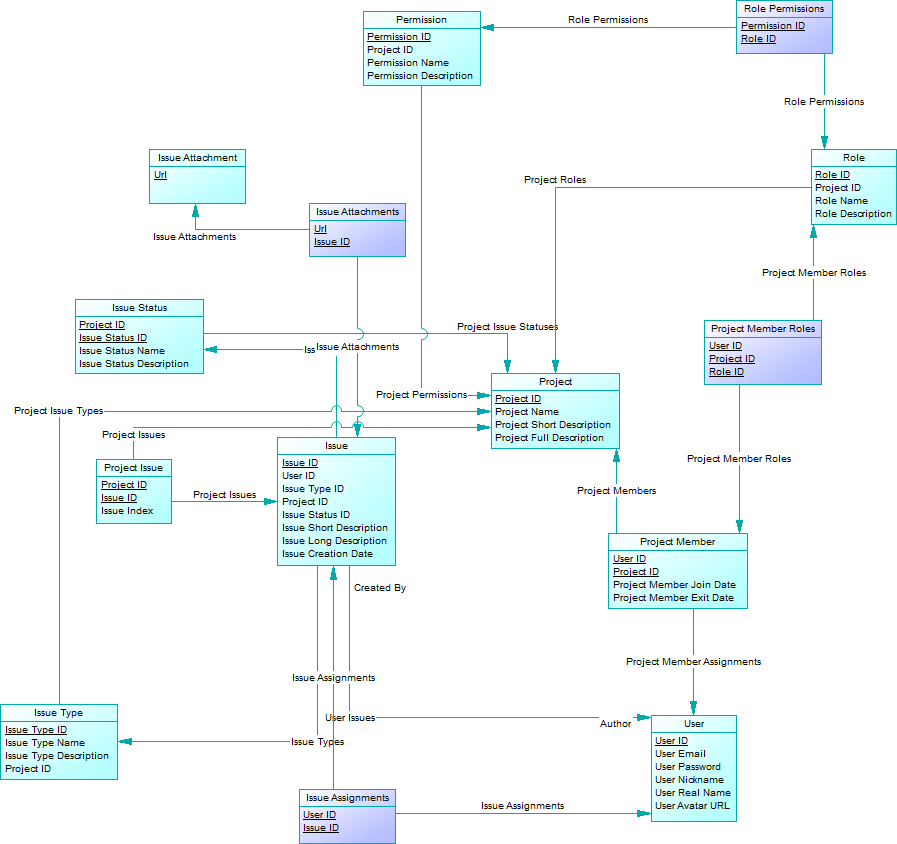
\includegraphics[width=1\textwidth]{4_db_physical}
			\caption{Фізична модель бази даних багтрекеру}
			\label{db_physical}
		\end{figure}
	
	\subsection{Розробка інтерфейсу користувача багтрекінгової системи}
		\subparagraph{Material Design.}
		
			Розробка інтерфейсу користувача велась з використанням гайдлайнів Material Design.\cite{material_design} Material Design дозволяє більш об'єктивно підходити до прийняття дизайн-рішень: як щось виглядає, як щось працює, як здійснюється анімація і так далі. Вона задає розумні рамки, але не зайві обмеження.
			
			Material Design грунтується на чотирьох основних принципах:
			\begin{enumerate}
				\item Тактильні поверхні. У Material Design інтерфейс складається з відчутних шарів так званого «цифрової паперу». Ці шари розташовані на різній висоті і відкидають тіні один на одного, що допомагає користувачам краще розуміти анатомію інтерфейсу і принцип взаємодії з ним.
				\item Поліграфічний дизайн. Якщо вважати шари шматками «цифрового паперу», то в тому, що стосується «цифрового чорнила» (всього того, що зображується на «цифровому папері»), використовується підхід з традиційного графічного дизайну: наприклад, журнального і плакатного.
				\item Осмислена анімація. У реальному світі предмети не виникають нізвідки і не зникають в нікуди - таке буває тільки в кіно. Тому в Material Design ми весь час думаємо про те, як за допомогою анімації в шарах і в «цифрових чорнилах» давати користувачам підказки про роботу інтерфейсу.
				\item Адаптивний дизайн. Йдеться про те, як ми застосовуємо попередні три концепції на різних пристроях з різними дозволами і розмірами екранів.
			\end{enumerate}
			
			Як і в поліграфічному дизайні, в дизайні інтерфейсів колір є важливим засобом виразності. У колишньому Android колір був чимось додатковим, тепер же він грає більш помітну роль. У Material Design стандартна колірна палітра програми складається з основного і акцентного квітів. Основний використовується для великих областей на зразок action bar, а в його більш темну варіацію фарбується status bar. Більш яскравий акцентних колір використовується точково в елементах управління, кнопках, смужках, індикаторах і т.д. Акцентний колір покликаний привертати увагу користувача до ключових елементів, таким як плаваюча кнопка.
			
			У реальному світі об'єкти не можуть просто з'являтися з нізвідки або зникати в нікуди. Це викликало б подив і ставило людей у глухий кут. Тому і в Material Design осмислена анімація використовується, щоб показати, що саме тільки що сталося.
			
			Оскільки глибина інтерфейсу обмежена товщиною пристрою, всі трансформації об'єктів доводиться виробляти в площині. Це також призводить до того, що анімація трансформацій повинна бути асиметричною - тобто зміна ширини і висоти об'єкта має бути незалежним. В іншому випадку виникає ілюзія наближення або віддалення від глядача, причому на дуже велику відстань.
			
			Інший дуже важливий принцип анімації в Material Design - реакція на дії користувача. Там, де це можливо, епіцентром змін в інтерфейсі має бути дотик до екрану пристрою. Наприклад, хвиля, яка з'являється і йде від точки дотику пальцем. Цей ефект без проблем реалізується в Android L.
			
			І останній, ключовий принцип анімації: рух має бути швидким і чітким. На відміну від банального прискорення на початку і уповільнення в кінці крива анімації в Material Design більш натуральна і цікава. Об'єкти швидше реагують і досягають цільового стану, різкіше повертаються назад, але трохи довше йдуть до стану спокою в кінці. В результаті користувачеві потрібно менше чекати (це менше дратує). При цьому там, де об'єкт вже вийшов зі сфери інтересів користувачів, він дозволяє собі поводитися більш природно.
			
			Рекомендується брати кратні пропорції для всіх елементів. Зокрема - вибирати розмір app bar значно зручніше, якщо робити його кратним: 1х, 2х, 3х. На смартфонах і планшетах цей розмір різний, але додаток без проблем адаптується.
			
			Дотрисуючись цих принципів було побудовано користувацький інтерфейс, що буде зрозумілим абсолютній більшості користувачів, а також не потребує багато ресурсів для впровадження послідовного користувацького інтерфейсу.
	
		\subparagraph{Екран авторизації та реєстрації.}
		
			Оскільки системою використовується метод авторизації, оснований на перевірці пари email-пароль, форма авторизації надає два поля введення: email та пароль. По натиску на кнопку ''Sign in'' відбудеться авторизація.
			
			В разі необхідності реєстрації нового аккаунта в системі, користувач може натиснути на перемикач ''New user'' - ця дія призведе до появи форми реєстрації. Окрім полей для введення email та паролю, форма реєстрації також містить поля для введення нікнейму та реального імені користувача.
			
			Зовнішній вигляд процесу авторизації та реєстрації зображено в додатках \ref{scr_ui_auth} та \ref{scr_ui_signup}.
	
		\subparagraph{Екран списку проектів.}
		
			Одразу після аторизації користувач перенаправляється на екран списку проектів. На ньому він може побачити список проектів, в яких він примає участь та їх короткий опис. Також, на цьому екрані користувач може виконати вихід із системи та створити новий проект (якщо він має на це право). Кнопка, що дозволяє перейти до створення нового проекту з'являється лише у тому випадку коли у користувача достатньо прав для створення проекту.
			
			Зовнішній вигляд екрану списку проектів зображено в додатку \ref{scr_ui_projects_list}.
			
		\subparagraph{Екран створення нового проекту.}
		
			Користувач, що натиснув на кнопку створення нового проекту буде перенаправлений на екран створення проекту. На цьому екрані користувач має ввести дані щодо проекту, такі як: назва проекту, короткий опис, повний опис. Для створення нового проекту, після введення необхідних даних користувачу потрібно натиснути кнопку ''Create''. Також, якщо користувач передумав створювати новий проект - в будь який момент він може натиснути кнопку ''Cancel'', цим самим відмінивши створення проекту.
			
			Зовнішній вигляд екрану створення проекту зображено в додатку \ref{scr_ui_project_creation}.
	
		\subparagraph{Екран проекту.}
		
			Користувач, що натиснув на деякий проект зі списку проектів буде перенаправлений на екран цього проекту. На даному екрані він може продивитись інформацію щодо проекту, його автора, учасників з їх ролями в межах проекту, та звіти, пов'язані з цим проектом. Також, якщо користувач має на це право, по натиску на кнопку ''Edit'' він може відредагувати інформацію щодо проекту та додати або видалити учасника.
			
			Зовнішній вигляд екрану проекту зображено в додатках \ref{scr_ui_project_1}, \ref{scr_ui_project_2} та \ref{scr_ui_project_edit}.
	
		\subparagraph{Екран додавання учасника проекту.}
		
			Якщо користувач, що має право на додавання нового учасника проекту, при редагуванні проекту натисне на кнопку ''Add'' - його буде перенаправлено на екран додавання нового учасника проекту. Першим етапом додавання учасника до проекту є його вибір зі списку користувачів в системі. Другим етапом є вибір ролі для попередньо обраного учасника. Після вибора ролі нового учасника проекту стане активною кнопка ''Add''. По натиску на неї буде додано нового учасника до проекту. Також, в будь-який момент користувач може відмінити додавання нового учасника проку натиском на кнопку ''Cancel''.
			
			Зовнішній вигляд екрану додавання нового учаснику проекту зображено в додатках \ref{scr_ui_add_project_members_1} та \ref{scr_ui_add_project_members_2}.
	
		\subparagraph{Екран звіту.}
		
			При натисканні на будь-який елемент списку звітів на екрані проекту користувача буде перенаправлено на екран звіту. На даному екрані він може продивитись опис проблеми, представленої в звіті, його автора, тип, статус, відповідальну особу а також додатки.
			
			Якщо у користувача є право на редагування даного звіту, для нього буду відображено кнопку ''Edit''. По натиску на цю кнопку користувач зможе відредагувати опис звіту, його тип та додатки. Також, при наявності на це права, користувач може змінити статус звіту та відповідальну особу.
			
			Зовнішній вигляд екрану звіту зображено в додатках \ref{scr_ui_issue_1}, \ref{scr_ui_issue_2} та \ref{scr_ui_issue_edit}.

% \subsection{Опис розробки програмних компонентів} - Ain't nobody got time fot that

\section{Тестування багтрекеру}

	Програм без помилок не існує. Практика доводить, що винуватцями помилок у програмах найчастіше бувають самі програмісти. Один із загальних законів практичного програмування полягає в тому, що жодна програма не дає бажаних результатів при першій спробі трансляції та виконання.~\cite{fast_testing}
	
	Техніка тестування включає як процес пошуку помилок або інших дефектів, так і випробування програмних складових з метою оцінки. Може оцінюватись:
	\begin{itemize}
		\item відповідність вимогам, якими керувалися проектувальники та розробники;
		\item правильна відповідь для усіх можливих вхідних даних;
		\item виконання функцій за прийнятний час;
		\item практичність;
		\item сумісність з програмним забезпеченням та операційними системами;
		\item відповідність задачам замовника.
	\end{itemize}
	
	Оскільки число можливих тестів навіть для нескладних програмних компонент практично нескінченне, тому стратегія тестування полягає в тому, щоб провести всі можливі тести з урахуванням наявного часу та ресурсів. Як результат програмне забезпечення (ПЗ) тестується стандартним виконанням програми з метою виявлення багів (помилок або інших дефектів).~\cite{software_testing}
	
	Тестування ПЗ може надавати об'єктивну, незалежну інформацію про якість ПЗ, ризики відмови, як для користувачів так і для замовників.~\cite{agile_testing}
	
	% LOL begin
	Окрім загальновідомої техніки TDD (Test Driven Development) існує також і техніка JDD (Jesus Driven Development).~\cite{jdd} Основною перевагою JDD перед TDD є опціональність слідування циклу ''Red-Green-Refactor''. Оскільки час виконання виконання дипломної роботи досить обмежений, було вирішено використовувати в розробці саме техніку JDD.
	% LOL end
	
	Оскільки в багтрекінговій системі найважливіша частина - сервер, а клієнтська сторона є просто методом введення-виведення даних для користувача, то основна маса автоматизованих інтеграційних тестів була написана саме для сервера.
	
	В ролі виконувача тестів було використано Mocha. В ролі тестового фреймворку було використано Should.js. Автоматизованими інтеграційними тестами було покрито усі основні операції по взаємодії з сервером. Результат виконання тестів зображено на рисунку \ref{test_results}. Після підтвердження проходження автоматизованих тестів також було виконано серію ручних тестів для того щоб впевнитись, що Android клієнт коректно взаємодіє з серверною частиною - для цього було вручну пройдено по всім екранам клієнтського додатку та перевірено працездатність системи у випадку взаємодії з сервером на цих екранах.
	
	\begin{figure}[H]
		\centering
		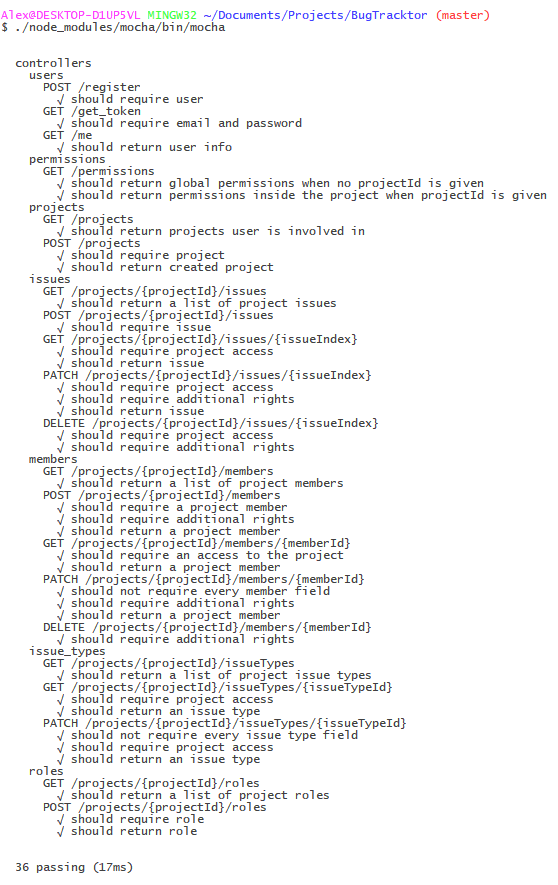
\includegraphics[width=0.6\textwidth]{5_mocha_results}
		\caption{Результат виконання автоматизованих тестів багтрекеру}
		\label{test_results}
	\end{figure}

\section{Висновки до третього розділу}

	У цьому розділі було наголошено на особливостях реалізації тих проектних рішень та вимог, що було сформовано у попередніх розділах. Для серверної частини було обрано мову програмування JavaScript на платформі Node.js та середовище розробки Atom. Такий вибір інструментів реалізації серверної частини було продиктовано зручністю їх використання в парі з JSON та фреймворком для специфікацій Swagger. Для клієнтського додатку під Android було обрано мову Java та середовище розробки Android Studio. Вибір саме цих інструментів реалізації клієнтської Android частини було продиктовано стандартами розробки під дану платформу.
	
	В межах розробки серверної частини системи було розроблено, впроваджено і протестовано механізми реакцій на запити користувацького додатку та механізми взаємодії з базою даних. Протягом усього періоду розробки виконувались автоматизовані тести для виявлення проблем на ранньому етапі.
	
	В межах розробки клієнтського Android додатку було розроблено і протестовано користувацький інтерфейс взаємодії з багтрекером. Після завершення розробки основного функціоналу клієнтської та серверної частини було проведено ручне тестування для того, щоб перепоканится, що система працює правильно.
	
	Ручне тестування багтрекінгової системи пройшло вдало, очікувані результати під час тестування співпадали з результатами виконня системи.

\end{document}